\section{KPP models}
\subsection{Author and source}
KPP - Kinetic preprocessor is a software tool that can be used to model chemical kinetics. It takes the specification of a chemical mechanism in a prescribed format and generates code to simulate the mechanism. More details about KPP itself can be found in the following papers \cite{Damian_2002}, \cite{Sandu_2003}, \cite{Daescu_2003} and \cite{Sandu_2006}. KPP can be obtained from \href{http://people.cs.vt.edu/~asandu/Software/Kpp/}{here}. The manual \cite{Sandu_2005} explains in great depth the usage of KPP.
\subsection{Description of the mathematical formulation}
The models that were generated using KPP are in effect a system of ODEs. A system of ODEs can be written mathematically as follows.

\[x' = f(t, x), \; t_0 \leq t \leq t_F, \; x(t_0) = x_0\]


\noindent Furthermore, these systems are usually stiff and will need an implicit integrator to handle the stiffness. Implicit integrators are written as:

\[x_{n+1} \,=\,  x_n \,+\, h \; \phi(t, x_n, x_{n+1}, h)\]

\noindent In order to solve for $x_{n+1}$ a root finding method such as Newton-Raphson iteration can be used. The jacobian of the RHS function ($f$) is then needed with respect to the variables $x$ to perform the newton iterations. \\

\noindent Directory structure and description of files follow on the next page.
\clearpage
\subsection{Directory structure and description of files}
The KPP models are organized into two directories with additional sub-directories as shown below:\\
\dirtree{%
.1 /. 
.2 small\_f90\_kpp\DTcomment{Directory containing KPP example small\_f90}. 
.3 small\_f90\_kpp/KPP\_generated\_jacobian \ldots{} \begin{minipage}[t]{5cm}
This directory contains the original files generated using KPP for the small\_f90 example{.}
\end{minipage}. 
.3 small\_f90\_kpp/OpenAD\_generated\_jacobian/ForwardVector.\ldots{} \begin{minipage}[t]{3cm}
This directory replaces KPPs Jacobian with that from OpenAD for the small\_f90 example{.}
\end{minipage}. 
.2 saprc\_f90\_kpp\DTcomment{Directory containing KPP example saprc\_f90}. 
.3 saprc\_f90\_kpp/KPP\_generated\_jacobian\ldots{} \begin{minipage}[t]{5cm}
This directory contains the original files generated using KPP for the saprc\_f90 example{.}
\end{minipage}.  
.3 saprc\_f90\_kpp/OpenAD\_generated\_jacobian/ForwardVector\ldots{} \begin{minipage}[t]{3cm}
This directory replaces KPPs Jacobian with that from OpenAD for the saprc\_f90 example{.}
\end{minipage}.  
}
\subsubsection{\texttt{KPP} generated jacobian}
The directory \texttt{KPP\_generated\_jacobian} in each of the example directories contains the unmodified code generated by \texttt{KPP}. A detailed description of the files can be found in the manual \cite{Sandu_2005}

\subsubsection{\texttt{OpenAD} generated jacobian}
The directory \texttt{OpenAD\_generated\_jacobian} replaces the KPP generated jacobian with the one generated by \texttt{OpenAD} in forward-vector mode. More details of the forward-vector mode can be found in \cite{Utke_2014}\\

\noindent The directory \texttt{OpenAD\_generated\_jacobian} contains the files to compile the binaries \texttt{small\_f90.exe}/\texttt{saprc\_f90.exe} 
%adjoint version of the optimal control problem listed in \ref{power_cont_adj_math} and \cite{Rao_2013}. The binaries (\textbf{files}), corresponding to these, on building the directory are \texttt{powergrid} (\textbf{{main.f90}}).\\

%\clearpage
%\begin{figure}[h]
%\centering
%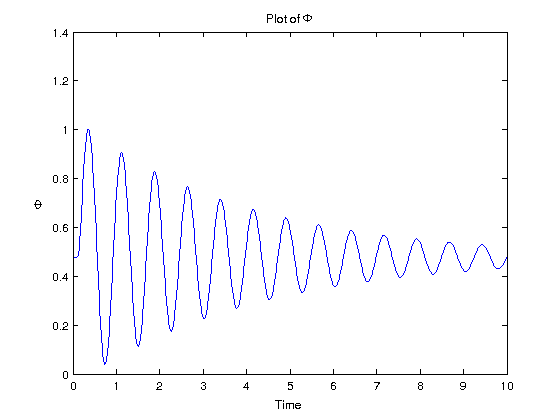
\includegraphics[width=1.2\linewidth]{../Code/miniApps/power_grid/phi_fortran_ca.png}
%\label{fig:plot_of_phi_fortran_ca}
%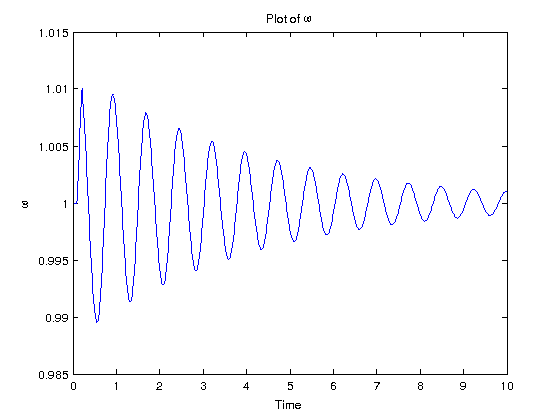
\includegraphics[width=1.2\linewidth]{../Code/miniApps/power_grid/omega_fortran_ca.png}
%\label{fig:plot_of_omega_fortran_ca}
%\end{figure}
%\clearpage
%\subsection{Modifications performed}
\subsection{How to build}
%Running make as below, in each of the five subdirectories beginning with \texttt{Fortran/} will build the  binary \texttt{powergrid}
%\hfill\break
%\begin{lstlisting}[language=mybash, numbers=none]
%    $ make
%\end{lstlisting}
\subsection{How to verify}
%At the time of writing, there exists no script that can validate the output from any of the binaries. All versions of the binary \texttt{powergrid} should produce similar (in some sense/nearby) optimal and objective values.\\
%
%\noindent Validation by eyeballing the output from each version of the binary  \texttt{powergrid} has been performed. 
%
%\begin{TodoPar}
%\noindent It will be valuable to write a \texttt{python} script that will take as input two \texttt{csv} files and find the \texttt{max-norm} of the difference between the corresponding entries. Other norms may also be computed. 
%\end{TodoPar}
%
%\begin{HypoPar}
%\noindent I wonder it might be difficult to test the derivatives of each version of \texttt{powergrid} against another, since the code does not do computations deterministically i.e. there are convergence related iterations, each version may take different trajectories (except at the starting point) until they arrive at nearby solutions that are similar as metioned earlier.\\
%
%\noindent One solution, might be to generate multiple experiments with several different starting points and compare the derivatives at the starting points alone.
%\end{HypoPar}


%\subsection{How to extend}
